
\documentclass[a4paper,12pt]{book}
\usepackage[utf8]{inputenc}
\usepackage[T1]{fontenc}
\usepackage[frenchb]{babel}
\usepackage{a4wide}
\usepackage{graphicx}
\graphicspath{{images/}}
\usepackage{subfig}
\usepackage{tikz}
\usetikzlibrary{shapes,arrows}
\usepackage{pgfplots}
\pgfplotsset{compat=newest}
\pgfplotsset{plot coordinates/math parser=false}
\newlength\figureheight
\newlength\figurewidth
\pgfkeys{/pgf/number format/.cd,
set decimal separator={,\!},
1000 sep={\,},
}
\usepackage{ifthen}
\usepackage{ifpdf}
\ifpdf
\usepackage[pdftex]{hyperref}
\else
\usepackage{hyperref}
\fi
\usepackage{color}
\hypersetup{%
colorlinks=true,
linkcolor=black,
citecolor=black,
urlcolor=black}

\renewcommand{\baselinestretch}{1.05}
\usepackage{fancyhdr}
\pagestyle{fancy}
\fancyfoot{}
\fancyhead[LE,RO]{\bfseries\thepage}
\fancyhead[RE]{\bfseries\nouppercase{\leftmark}}
\fancyhead[LO]{\bfseries\nouppercase{\rightmark}}
\setlength{\headheight}{15pt}

\let\headruleORIG\headrule
\renewcommand{\headrule}{\color{black} \headruleORIG}
\renewcommand{\headrulewidth}{1.0pt}
\usepackage{colortbl}
\arrayrulecolor{black}

\fancypagestyle{plain}{
  \fancyhead{}
  \fancyfoot[C]{\thepage}
  \renewcommand{\headrulewidth}{0pt}
}

\makeatletter
\def\@textbottom{\vskip \z@ \@plus 1pt}
\let\@texttop\relax
\makeatother

\makeatletter
\def\cleardoublepage{\clearpage\if@twoside \ifodd\c@page\else%
  \hbox{}%
  \thispagestyle{empty}%
  \newpage%
  \if@twocolumn\hbox{}\newpage\fi\fi\fi}
\makeatother

\usepackage{amsthm}
\usepackage{amssymb,amsmath,bbm}
\usepackage{array}
\usepackage{bm}
\usepackage{multirow}
\usepackage[footnote]{acronym}

\newcommand*{\SET}[1]  {\ensuremath{\mathbf{#1}}}
\newcommand*{\VEC}[1]  {\ensuremath{\boldsymbol{#1}}}
\newcommand*{\FAM}[1]  {\ensuremath{\boldsymbol{#1}}}
\newcommand*{\MAT}[1]  {\ensuremath{\boldsymbol{#1}}}
\newcommand*{\OP}[1]  {\ensuremath{\mathrm{#1}}}
\newcommand*{\NORM}[1]  {\ensuremath{\left\|#1\right\|}}
\newcommand*{\DPR}[2]  {\ensuremath{\left \langle #1,#2 \right \rangle}}
\newcommand*{\calbf}[1]  {\ensuremath{\boldsymbol{\mathcal{#1}}}}
\newcommand*{\shift}[1]  {\ensuremath{\boldsymbol{#1}}}

\newcommand{\eqdef}{\stackrel{\mathrm{def}}{=}}
\newcommand{\argmax}{\operatornamewithlimits{argmax}}
\newcommand{\argmin}{\operatornamewithlimits{argmin}}
\newcommand{\ud}{\, \mathrm{d}}
\newcommand{\vect}{\text{Vect}}
\newcommand{\sinc}{\ensuremath{\mathrm{sinc}}}
\newcommand{\esp}{\ensuremath{\mathbb{E}}}
\newcommand{\hilbert}{\ensuremath{\mathcal{H}}}
\newcommand{\fourier}{\ensuremath{\mathcal{F}}}
\newcommand{\sgn}{\text{sgn}}
\newcommand{\intTT}{\int_{-T}^{T}}
\newcommand{\intT}{\int_{-\frac{T}{2}}^{\frac{T}{2}}}
\newcommand{\intinf}{\int_{-\infty}^{+\infty}}
\newcommand{\Sh}{\ensuremath{\boldsymbol{S}}}
\newcommand{\C}{\SET{C}}
\newcommand{\R}{\SET{R}}
\newcommand{\Z}{\SET{Z}}
\newcommand{\N}{\SET{N}}
\newcommand{\K}{\SET{K}}
\newcommand{\reel}{\mathcal{R}}
\newcommand{\imag}{\mathcal{I}}
\newcommand{\cmnr}{c_{m,n}^\reel}
\newcommand{\cmni}{c_{m,n}^\imag}
\newcommand{\cnr}{c_{n}^\reel}
\newcommand{\cni}{c_{n}^\imag}
\newcommand{\tproto}{g}
\newcommand{\rproto}{\check{g}}
\newcommand{\LR}{\mathcal{L}_2(\SET{R})}
\newcommand{\LZ}{\ell_2(\SET{Z})}
\newcommand{\LZI}[1]{\ell_2(\SET{#1})}
\newcommand{\LZZ}{\ell_2(\SET{Z}^2)}
\newcommand{\diag}{\operatorname{diag}}
\newcommand{\noise}{z}
\newcommand{\Noise}{Z}
\newcommand{\filtnoise}{\zeta}
\newcommand{\tp}{g}
\newcommand{\rp}{\check{g}}
\newcommand{\TP}{G}
\newcommand{\RP}{\check{G}}
\newcommand{\dmin}{d_{\mathrm{min}}}
\newcommand{\Dmin}{D_{\mathrm{min}}}
\newcommand{\Image}{\ensuremath{\text{Im}}}
\newcommand{\Span}{\ensuremath{\text{Span}}}

\newtheoremstyle{break}
  {11pt}{11pt}%
  {\itshape}{}%
  {\bfseries}{}%
  {\newline}{}%
\theoremstyle{break}

%\theoremstyle{definition}
\newtheorem{definition}{Définition}[chapter]

%\theoremstyle{definition}
\newtheorem{theoreme}{Théorème}[chapter]

%\theoremstyle{remark}
\newtheorem{remarque}{Remarque}[chapter]

%\theoremstyle{plain}
\newtheorem{propriete}{Propriété}[chapter]
\newtheorem{exemple}{Exemple}[chapter]

\parskip=5pt
%\sloppy

\begin{document}

%%%%%%%%%%%%%%%%%%
%%% First page %%%
%%%%%%%%%%%%%%%%%%

\begin{titlepage}
\begin{center}


\includegraphics[width=0.6\textwidth]{entete}\\[1cm]

{\large Master 2 multimédia, Université de Bourgogne}\\[0.5cm]

{\large Rapport de stage de fin d'études}\\[0.5cm]

% Title
\rule{\linewidth}{0.5mm} \\[0.4cm]
{ \huge \bfseries Chargé de communication autour du projet PnS.com \\[0.4cm] }
\rule{\linewidth}{0.5mm} \\[1.5cm]

% Author and supervisor
\noindent
\begin{minipage}{0.4\textwidth}
  \begin{flushleft} \large
    \emph{Auteur :}\\
    Mr. Bérenger \textsc{Thévenet}\\
  \end{flushleft}
\end{minipage}%
\begin{minipage}{0.4\textwidth}
  \begin{flushright} \large
    \emph{Encadrants :} \\
    Mme.~Sandrine \textsc{Lanquetin}\\
    Mr.~Joel \textsc{Savelli}\\
    Mr.~Olivier \textsc{Leick}
  \end{flushright}
\end{minipage}

\vfill

% Bottom of the page
{\large Version 0.9.2 du\\ \today}

\end{center}
\end{titlepage}

%%%%%%%%%%%%%%%%%%%%%%%%%%%%%
%%% Remerciments %%%
%%%%%%%%%%%%%%%%%%%%%%%%%%%%%

\frontmatter

%\chapter*{Remerciements}
%Je tiens à remercier toutes les personnes qui ont contribué au succès de mon stage et qui m'ont aidé lors de la rédaction de ce rapport.

%Tout d'abord, j'adresse mes remerciements à mon professeur, Mme.~Sandrine \textsc{Lanquetin} de l'Université de Bourgogne qui m'a permis de postuler dans cette entreprise.

%Je tiens à remercier vivement mon maitre de stage, Mr.~Olivier \textsc{Leick}, responsable solution au sein de l'entreprise Orange, pour son accueil, ses conseils, le temps passé ensemble et le partage de son expertise au quotidien ainsi que ses précieux conseils lors de la rédaction de ce rapport.

%Je remercie également toute l'équipe de la SDFY Orange pour leur accueil et leur esprit d'équipe.

%Enfin, je tiens à remercier toutes les personnes qui m'ont conseillé et relu lors de la rédaction de ce rapport de stage : ma famille, ma compagne Mélane, et mon amie Nilu.$

\clearpage
\tableofcontents

\clearpage
\listoffigures

\clearpage

%%%%%%%%%%%%%%%%%%%%%%%%%%%%%%%%%%%%%%%%%%%%%
%                 Accronymes                %
%%%%%%%%%%%%%%%%%%%%%%%%%%%%%%%%%%%%%%%%%%%%%
\chapter*{Liste des sigles et acronymes}

Liste des sigles et acronymes internes :\\

\begin{acronym}[CP-OFDMX]

\acro{DFY}{\emph{Data Factory}}
\acro{OKAPI}{\emph{Oauth2 Kerberos API}}
\acro{PnS}{\emph{Profile and Syndication}}
\acro{SDFY}{\emph{Smart Data Factory}}
\acro{SI}{\emph{Système d'Informations}}


\end{acronym}


Liste des sigles et acronymes techniques :\\

\begin{acronym}[CP-OFDMX]

\acro{API}{\emph{Application Programming Interface - Interface de programmation}}
\acro{SSO}{\emph{Signe Sign-On - Authentification unique}}
\acro{TTL}{\emph{Time To Live - Durée de vie }}

\end{acronym}

%%%%%%%%%%%%%%%%%%%%%%%%%%%%%%%%%%%%%%%%%%%%
%%% Content of the report and references %%%
%%%%%%%%%%%%%%%%%%%%%%%%%%%%%%%%%%%%%%%%%%%%

\mainmatter
\pagestyle{fancy}

\cleardoublepage

\chapter*{Introduction}
\addcontentsline{toc}{chapter}{Introduction}
\markboth{Introduction}{Introduction}
\label{chap:introduction}
%\minitoc

Avec 30 millions de clients mobile et plus de 18 millions de clients  pour le haut et très haut débit fixe, Orange est le premier opérateur en France et la 50\up{ième} entreprise la plus influente au monde en 2016. Avec une telle importance autant au niveau national qu'international, la firme se doit de rester innovante et à la pointe de la technologie pour pouvoir répondre aux besoins de plus en plus précis et diversifiés de leurs clients. La division que j’ai intégré, la Smart Data Factory (SDFY), opère sur plusieurs secteurs différents allant de la gestion de base de données à la recommandation personnalisée en passant par les application mobiles et la sécurité. Avec une telle diversité de secteurs d’activités, il n’est pas évident de tenir toutes les équipes au courant de toutes les nouveautés et avancées au sein de chaque projet ni de pouvoir les expliquer simplement et ludiquement aux personnes sans connaissances techniques.\\
<<<<<<< HEAD
L’offre de stage à laquelle j’ai répondu s’inscrit dans la lignée d’un projet qui avait été initié par un prestataire externe : pouvoir expliquer de manière compréhensible et divertissant sous forme de vidéos le fonctionnement et l’intérêt des nouvelles  interfaces de programmations (APIs) produites au sein de la SFDY dans le cadre du programme PnS.com, qui a pour but de fournir un stockage des données en libre service. J’ai choisi de répondre à cette offre car j’étais intéressé par le côté créatif de la réalisation de vidéos qui était une suite directe du cours de « Pratiques plastiques » que j’ai suivi cette année et qui m’a beaucoup intéressé. C’était aussi l’occasion pour moi de mettre en pratique les connaissances techniques acquises au cours de mes cinq années d'études à l’Université de Bourgogne.\\
=======
L’offre de stage à laquelle j’ai répondu s’inscrit dans la lignée d’un projet qui avait été initiée par un prestataire externe : pouvoir expliquer de manière compréhensible et divertissant sous forme de vidéos le fonctionnement et l’intérêt des nouvelles  interfaces de programmations (APIs) produites au sein de la SFDY dans le cadre du programme PnS.com, qui a pour but de fournir un stockage des données en libre service. J’ai choisi de répondre à cette offre car j’étais intéressé par le côté créatif de la réalisation de vidéos qui était une suite directe du cours de « Pratiques plastiques » que j’ai suivi cette année et qui m’a beaucoup plu. C’était aussi l’occasion pour moi de mettre en pratique les connaissances techniques acquises au cours de mes cinq années d'études à l’Université de Bourgogne.\\
>>>>>>> origin/master
Dans ce rapport, nous étudierons plus en détail l’entreprise et son secteur d’activité, puis nous nous concentrerons sur mon stage, en nous focalisant sur mes différentes missions puis mon bilan.
%%% Local Variables: 
%%% mode: latex
%%% TeX-master: "isae-report-template"
%%% End: 

\chapter{L'entreprise et son secteur d'activité}
\label{chap:premierchapitre}

\section{L'histoire d'Orange}


En juillet 1992, le premier opérateur mobile  de France voit le jour sous le nom Itineris. Deux ans plus tard Orange est lancée sur le marché britannique et devient le quatrième opérateur du pays. Orange est côté à la bourse de Londres et au NASDAQ en avril 1996. A ce moment, Orange possède environ 500 000 abonnés et un mois plus tard figure dans la liste des plus grandes entreprises britanniques. À la fin de l'année 1998 Orange compte plus d'1 million d'abonnés et a lancé une promesse de performance réseau. Au même moment, en France, Itineris couvre 97\% de la population avec 7 700 relais et compte 5,5 millions de clients. Un an plus tard, après avoir lancé le premier système de reconnaissance vocale mobile du Royaume Uni, Orange est racheteé par Mannesmann ce qui porte le nombre d'abonnés à plus de 3,5 millions. Quelques mois plus tard, Orange lance sa première plate forme internet mobile : "orange.net". En février 2000, alors que Mannesmann venait d'être rachetée, il est entrepris de vendre Orange qui sera reprise un mois plus tard par France Télécom. Les opérations de téléphonies mobiles de France Télécom sont donc fusionnées avec celles d'Orange, ce qui pousse le nouveau groupe "Orange S.A" \textit{(Société Anonyme)} à être présent dans 20 pays. Un an plus tard, en juin 2001, mobicarte, Ola et Itineris, qui compte alors plus de 10 millions de clients, fusionnent pour devenir le Orange que nous connaissons. En juin 2006, Orange rachète Wanadoo. En 2011, France Télécom communique en tant que "Groupe France Télécom - Orange" puis vote le changement de nom pour "Orange" en mai 2013.



\section{Secteur d'activité}

Avec la démocratisation d'internet et des objets reliés au web, nous sommes de plus en plus connectés. Avec plus de 3,5 milliards d'internautes, chiffre en perpétuelle hausse, et plus de 3h par jour passées devant l'écran de son téléphone, les milieux de la téléphonie et de l'internet doivent toujours être à l'écoute des besoins des clients pour pouvoir répondre à leurs demandes en constante évolution. Orange se donne pour but de répondre à chaque besoin, que cela soit une connectivité sans faille ou bien encore conseiller un bon rapport qualité/prix dans le but de proposer à chaque client la meilleure offre. À plus long terme, Orange souhaite proposes à ses clients des services numériques leur permettant de profiter de ce qui leur est essentiel. \\
Les principales activités d'Orange sont :\\
Une offre d'accès internet en haute débit, ADSL et fibre optique et des services multimédias via la Livebox, tels que la TV ou un système de vidéos à la demande. A ce jour, Orange compte 3,3 millions de clients de la fibre et plus de 11 millions pour le haut débit.\\
Orange fournit aussi des services mobiles sur des réseaux de 2, 3 et 4\up{ème} génération avec plus de 30 millions d'utilisateurs, ce qui place les place comme 1\up{er} opérateur mobile en France.\\
Orange propose aussi des applications permettant des transactions financières, "Orange Money", comptant plus de 29 millions de clients dans 17 pays. En avril dernier à été lancé "Orange Bank", un service ayant pour ambition d'être une banque mobile.


\section{La Digital Factory}

Au sein du groupe se trouve la Digital Factory (DFY) qui est une division ayant pour buts de développer et suivre de bout en bout des projets digitaux multi supports avec une grande capacité à innover et en se servant de technologies open-source et réutilisables telles que des interfaces de programmations (APIs). Pour ce faire, quatre principes sont mis en \oe{}uvre à la DFY :

\begin{itemize}
    \item Chercher à réduire la taille unitaire des projets, en itérant plusieurs fois avant 	d’atteindre l’objectif final
    \item Organiser les équipes par produit avec au moins un représentant métier
    \item Privilégier l’autonomie et la responsabilité des équipes
    \item Rechercher la proximité avec le marketing, en partageant les mêmes objectifs business et techniques
\end{itemize}

De manière plus précise, la DFY est en charge de développer et de maintenir les services du portail Orange, comprenant entre autre le site orange.fr, les chaînes, les applications mail,  les logiciels développés par Orange.
Elle est également responsable de domaines plus sensibles comme la sécurité, les projets ainsi que la gestion et le traitement des données.\\

La DFY regroupe en son sein 400 développeurs pour 8 salles d’hébergement comprenant 3200 serveurs traitant 21 Gb de données par seconde et 350 000 requêtes "http" par seconde en pics provoqués par plus de 25 millions de visiteurs par jour sur le portail Orange.

Cette entité regroupe plusieurs centres de compétences telles que le développement "tout écrans" et périphériques, l'ergonomie et design, l'hébergement et la supervision, le data science, la sécurité et la gestion de projet. Tous ces secteurs étant gérés de manière agile et en DevOps. 

%%% Local Variables: 
%%% mode: latex
%%% TeX-master: "isae-report-template"
%%% End: 
\chapter{Mon stage}
\label{sec:unchapitre}

Lorsque j'ai répondu à l'offre de stage, il été avait initialement prévu que je produise une newsletter ainsi que trois vidéos sur trois APIs différentes qui sont :

\begin{itemize}
    \item Gat'Ape/Okapi
    \item Zbus
    \item Valkey
\end{itemize}

Cependant, aux vues de mon avancement et de l'intérêt suscité par les vidéos produites, j'ai accepté de travailler sur trois autres projets :

\begin{itemize}
    \item Explication des difficultés liées à la création et à la publication d'APIs avant l'arrivée du cloud au sein d'Orange
    \item Présentation des avantages du travail en DevOps
    \item Promotion de PnS.com
\end{itemize}



Les vidéos traitant des APIs se devaient d'être vulgarisées et simple à comprendre étant donné qu'elles pourraient être destinés à un public très vaste. Chaque vidéo se doit d'être compréhensible par un programmeur ou un manager par exemple. La principale difficulté est de devoir vulgariser un maximum tout en gardant des précision pour qu'elles restent pertinentes pour les personnes les plus techniques. La diffusion de ces vidéos peut se faire pour montrer les dernières avancées au sein de la SDFY, ou encore pour promouvoir un produit, ou le proposer à des clients en tant que nouvelle solution. \\

En revanche, l'approche pour les 3 autres vidéos est totalement différente, elles s'adressent à un public ciblé et ont principalement un but promotionnel. Deux de ces vidéos ont été réalisées pour un événement particulier. \\



\section{Style de vidéo et choix du logiciel}
Comme précisé dans l'introduction, mon stage est la suite d'un projet de série de vidéos ayant été commencées par un prestataire externe. La première vidéo avait été faite en scribing, sorte de présentation sur tableau blanc animé avec une main tenant un crayon qui va dessiner les éléments. J'ai volontairement choisi de ne pas réutiliser ce style car il peut s'avérer très répétitif et ennuyeux sur le long terme.

\begin{figure}[htp]
  \centering
  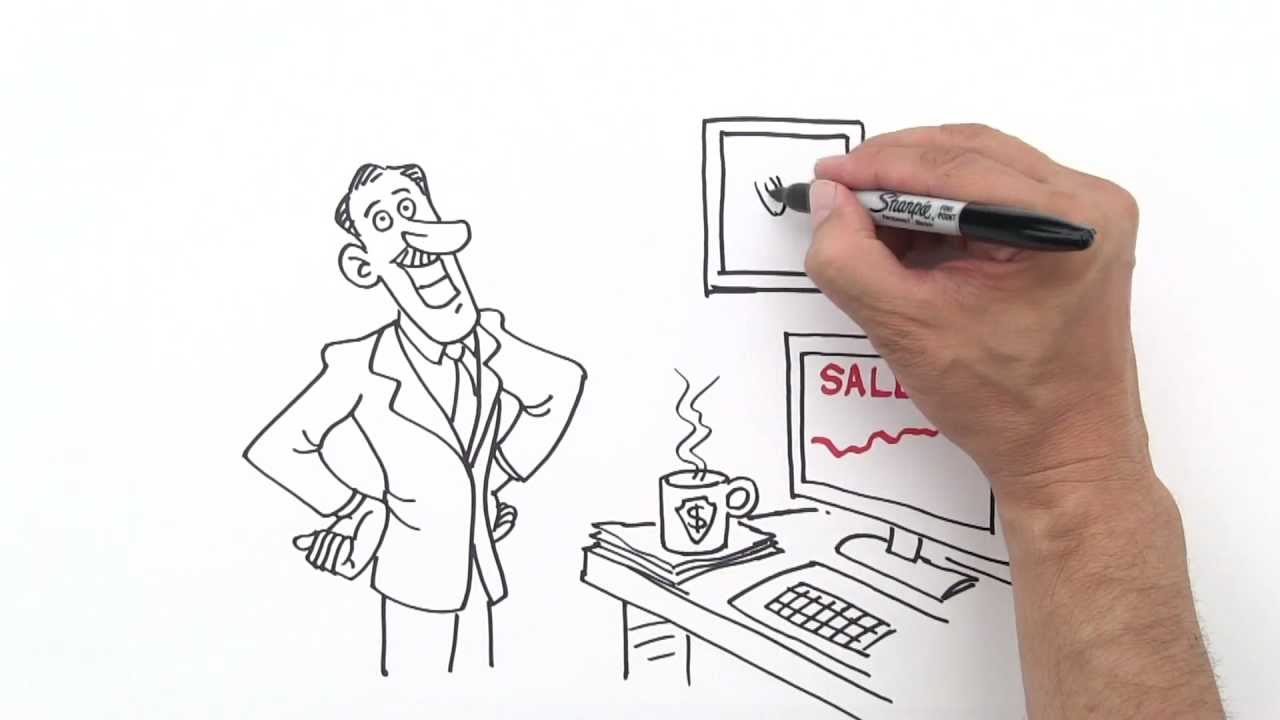
\includegraphics[width=15cm]{images/scribe}
  \caption{Exemple d'une vidéo de type scribing.}
  \label{scribe}
\end{figure}

J'ai opté pour un thème moderne et minimaliste pour que les spectateurs ne se perdent pas dans les détails. Un fond blanc ou gris clair et les illustrations trouvées sur le site de la marque. De cette manière j'étais sûr de respecter les conditions de la charte graphique, à savoir, au mois 20\% de couleur orange sur les illustrations ainsi que les couleurs et la police de caractères officielle. J'ai du cependant détourer certaines images, en créer certaines tels les enveloppes visibles dans la légende \textbf{AJOUTER LE NUMERO DE LA LEGENDE}. En ce qui concerne le logiciel, je me suis servi de Adobe After Effects CC, logiciel que j'avais déjà expérimenté à titre personnel et dont j'ai reçu une formation lors d'un de mes cours du premier semestre. After Effects CC est un logiciel très complet qui permet d'animer des objets de manière précise en ayant la main mise sur tous les paramètres, ce qui permet une création quasiment sans restriction dans un environnement dans lequel j'avais déjà des repères.

\section{Organisation}
Le processus de création de chaque vidéo est découpé en plusieurs phases qui ont toujours lieu dans cet ordre :\\

Si la vidéo était un projet prévu à l'avance, ce qui était le cas pour les trois vidéos traitant les APIs, je commençais par lire de la documentation pour me renseigner sur ce que propose le produit et son utilité.\\

Avait ensuite lieu une réunion avec le chef de projet du sujet de la vidéo ainsi que une ou deux autres personnes également concernées (programmeur, graphiste). Lors de cette réunion, je cherchais à comprendre les poins important à développer dans la vidéo ainsi que messages à faire passer. Si besoin, je demandais également des précisions sur le produit. Une fois les idées et les messages principaux réunis, nous faisons ensemble le tri pour ne garder que les idées les plus pertinentes pour le public ciblé.\\





\begin{figure}[htp]
  \centering
  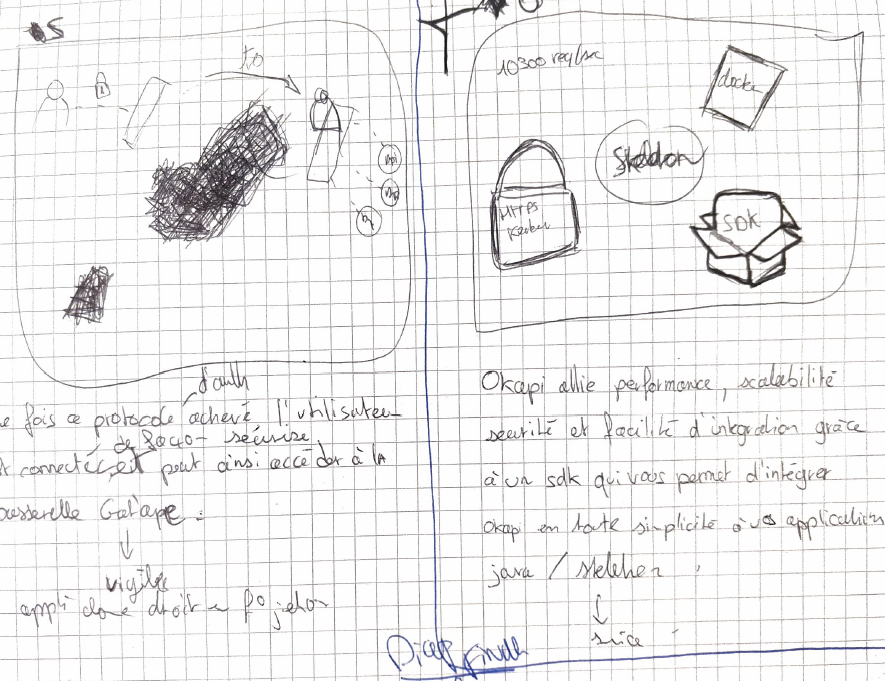
\includegraphics[width=15cm]{images/sb/sb1}
  \caption{Une page du storyboard de la vidéo Gat'ape/Okapi.}
  \label{sbzbus}
\end{figure}




Lorsque le choix est définitif et approuvé par tout le monde, je travaille sur un storyboard et un script qui permettront de se rendre compte de la mise en page et du texte énoncé. 


Une fois ces deux éléments achevés, je les envoie aux personnes présentes lors de la réunion pour avoir leur retour et impressions. S'il y avait des modifications majeures qui nécessitait une nouvelle phase de vérification, je renvoyais de nouveau le storyboard et le script.\\


Une fois le script validé, je pouvais commencer la création de la vidéo en animant les éléments prévus au storybaord pour garder un ensemble dynamique. J'ai un maximum mis en mouvement les éléments importants sans trop animer la totalité pour que le spectateur puisse se concentrer sur la future voix off. Une fois les animations terminées, j'enregistre la voix off en lisant le script préalablkement écrit puis je la synchronise avec les animations. Pour finir, j'ajoute une musique de fond, pour combler les blancs de manière conviviale.\\

Une fois ceci fait j'envoie ce pilote aux personnes concernées en attendant leurs remarques éventuelles. S'il y a besoin de modifier des parties, je le fais puis leur renvoie la nouvelle version jusqu'à validation de la vidéo.


%Avant de développer le contexte et la production de chaque vidéo, je vais d'abord présenter le programme PnS.com et ses différents composants. 

\section{Présentation générale de l'écosystème PnS.com}


PnS.com est une extension de l'ancienne solution de stockage de données à haute performance et disponibilité appelé PnS. Cette extension le rend As A Service (AAS), c'est à dire accessible via internet par le client. L'architecture de PnS.com se divise en quatre parties.

\begin{itemize}
    \item Le backend
    \item Les injecteurs
    \item Le backoffice
    \item Les APIs
\end{itemize}

%%%%%%%%%%
% Schema %
%%%%%%%%%%

\begin{figure}[htp]
  \centering
  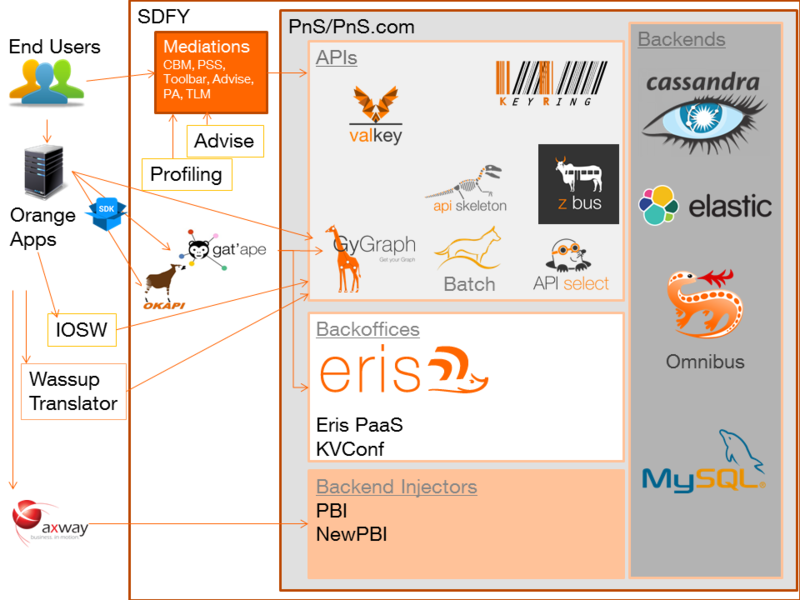
\includegraphics[width=15cm]{images/pns/psn.png}
  \caption{Schéma de l'architecture de PnS.com.}
  \label{pns}
\end{figure}


Le backend est composé de la base de donnée Cassandra noSQL, prévue pour stocker un grand nombre de données stockées sur plusieurs serveurs différents. Elle possède donc une haute disponibilité et possède un système d'élimination de ponts défaillants qui lui assure une quasi certitude d'accès aux données. Parmi le backend figure aussi Elastic Search qui est un moteur de recherche qui va faciliter la consultation de la base de donnée, et Omnibus sert de lien entre Cassandra et Elastic Search.\\

Les injecteurs quant à eux, ont le rôle d'envoyer en masse des informations dans la base de données.\\

Le backoffice, et plus particulièrement Eris, qui est l'outil de gestion des flux. Il permet à un service de type PnS de présenter l'ensemble de ses relations avec ses fournisseurs et ses partenaires. Ses principales fonctionnalités sont de pouvoir rechercher de l'information par mot clef, mais aussi de saisir de l'information et de pouvoir suivre les flux.\\

Enfin, les APIs sont présentes pour ajouter des fonctionnalités à l'écosystème PnS.com. Parmi ces APIs, nous retrouvons Batch, qui va permettre des injections, Select, qui va permettre de faire des recherches sous forme de texte comme nous le ferions dans un moteur de recherche au lieu d'utiliser les noms des variables. Skeleton, socle pour les APIs, Zbus, dont le but est de transmettre des messages \textit{(cf : 2.3)}, GyGraph qui permet de modéliser une base de donnée sous forme de graphe et Valkey qui fournit le modèle clef/valeur \textit{(cf : 2.4)}.\\

Actuellement, 185 applications se connectent à PnS quotidiennement, ce qui représente 20 000 requêtes/s en lecture et 8 000 requêtes/s en lecture sur la base de données. Ces applications viennent de milieux différents tels que le portail orange.fr, encore l'espace client ou bien encore le Suivi Conso par exemple. Ces applications viennes chercher des données, que cela soit les leurs ou bien des données provenant de référentiels, ou bien une grande capacité de stockage et une scalabilité sans impact. En effet, PnS dispose de 70TB qui permettent d'absorber les variations de volume de stockage.

\section{Vidéo sur Gat'Ape/Okapi}

\subsection{Contexte}
Gat'ape/Okapi est une API faisant partie de l'écosystème PnS.com qui permet d'exposer, de s'authentifier et de sécuriser les APIs de cet écosystème. Gat'ape et Okapi ont deux fonctions bien distinctes.\\

Okapi est le système d'authentification qui va permettre la connexion aux autres APIs. Okapi est basé sur le couple Oauth2/Kerberos qui va permettre une identité indépendante à chaque entité tout en offrant un système d'authentification unique (SSO) qui va permettre à l'utilisateur d'accéder à plusieurs applications en ne s'authentifiant qu'une seule fois. Cette authentification repose sur un système de clé secrète et de jeton. Il est à noter que des options de sécurité plus complexes sont aussi disponibles.\\

Gat'ape quant à elle est la passerelle qui va permettre d'exposer les APIs, c'est à dire, de les rendre visibles à d'autres utilisateurs pour qu'ils puissent s'y connecter. Gat'ape va pouvoir offrir un contrôle d'accès et un contrôle de trafic permettant de réguler le flux des utilisateurs. Gat'ape est également responsable  de l'authentification et de la sécurité lors de la consommation par Okapi. En plus de cela, gat'ape est également scalable, c'est à dire qu'elle va pouvoir maintenir son activité et sa performance même lors d'une forte demande.\\

\begin{figure}[htp]
  \centering
  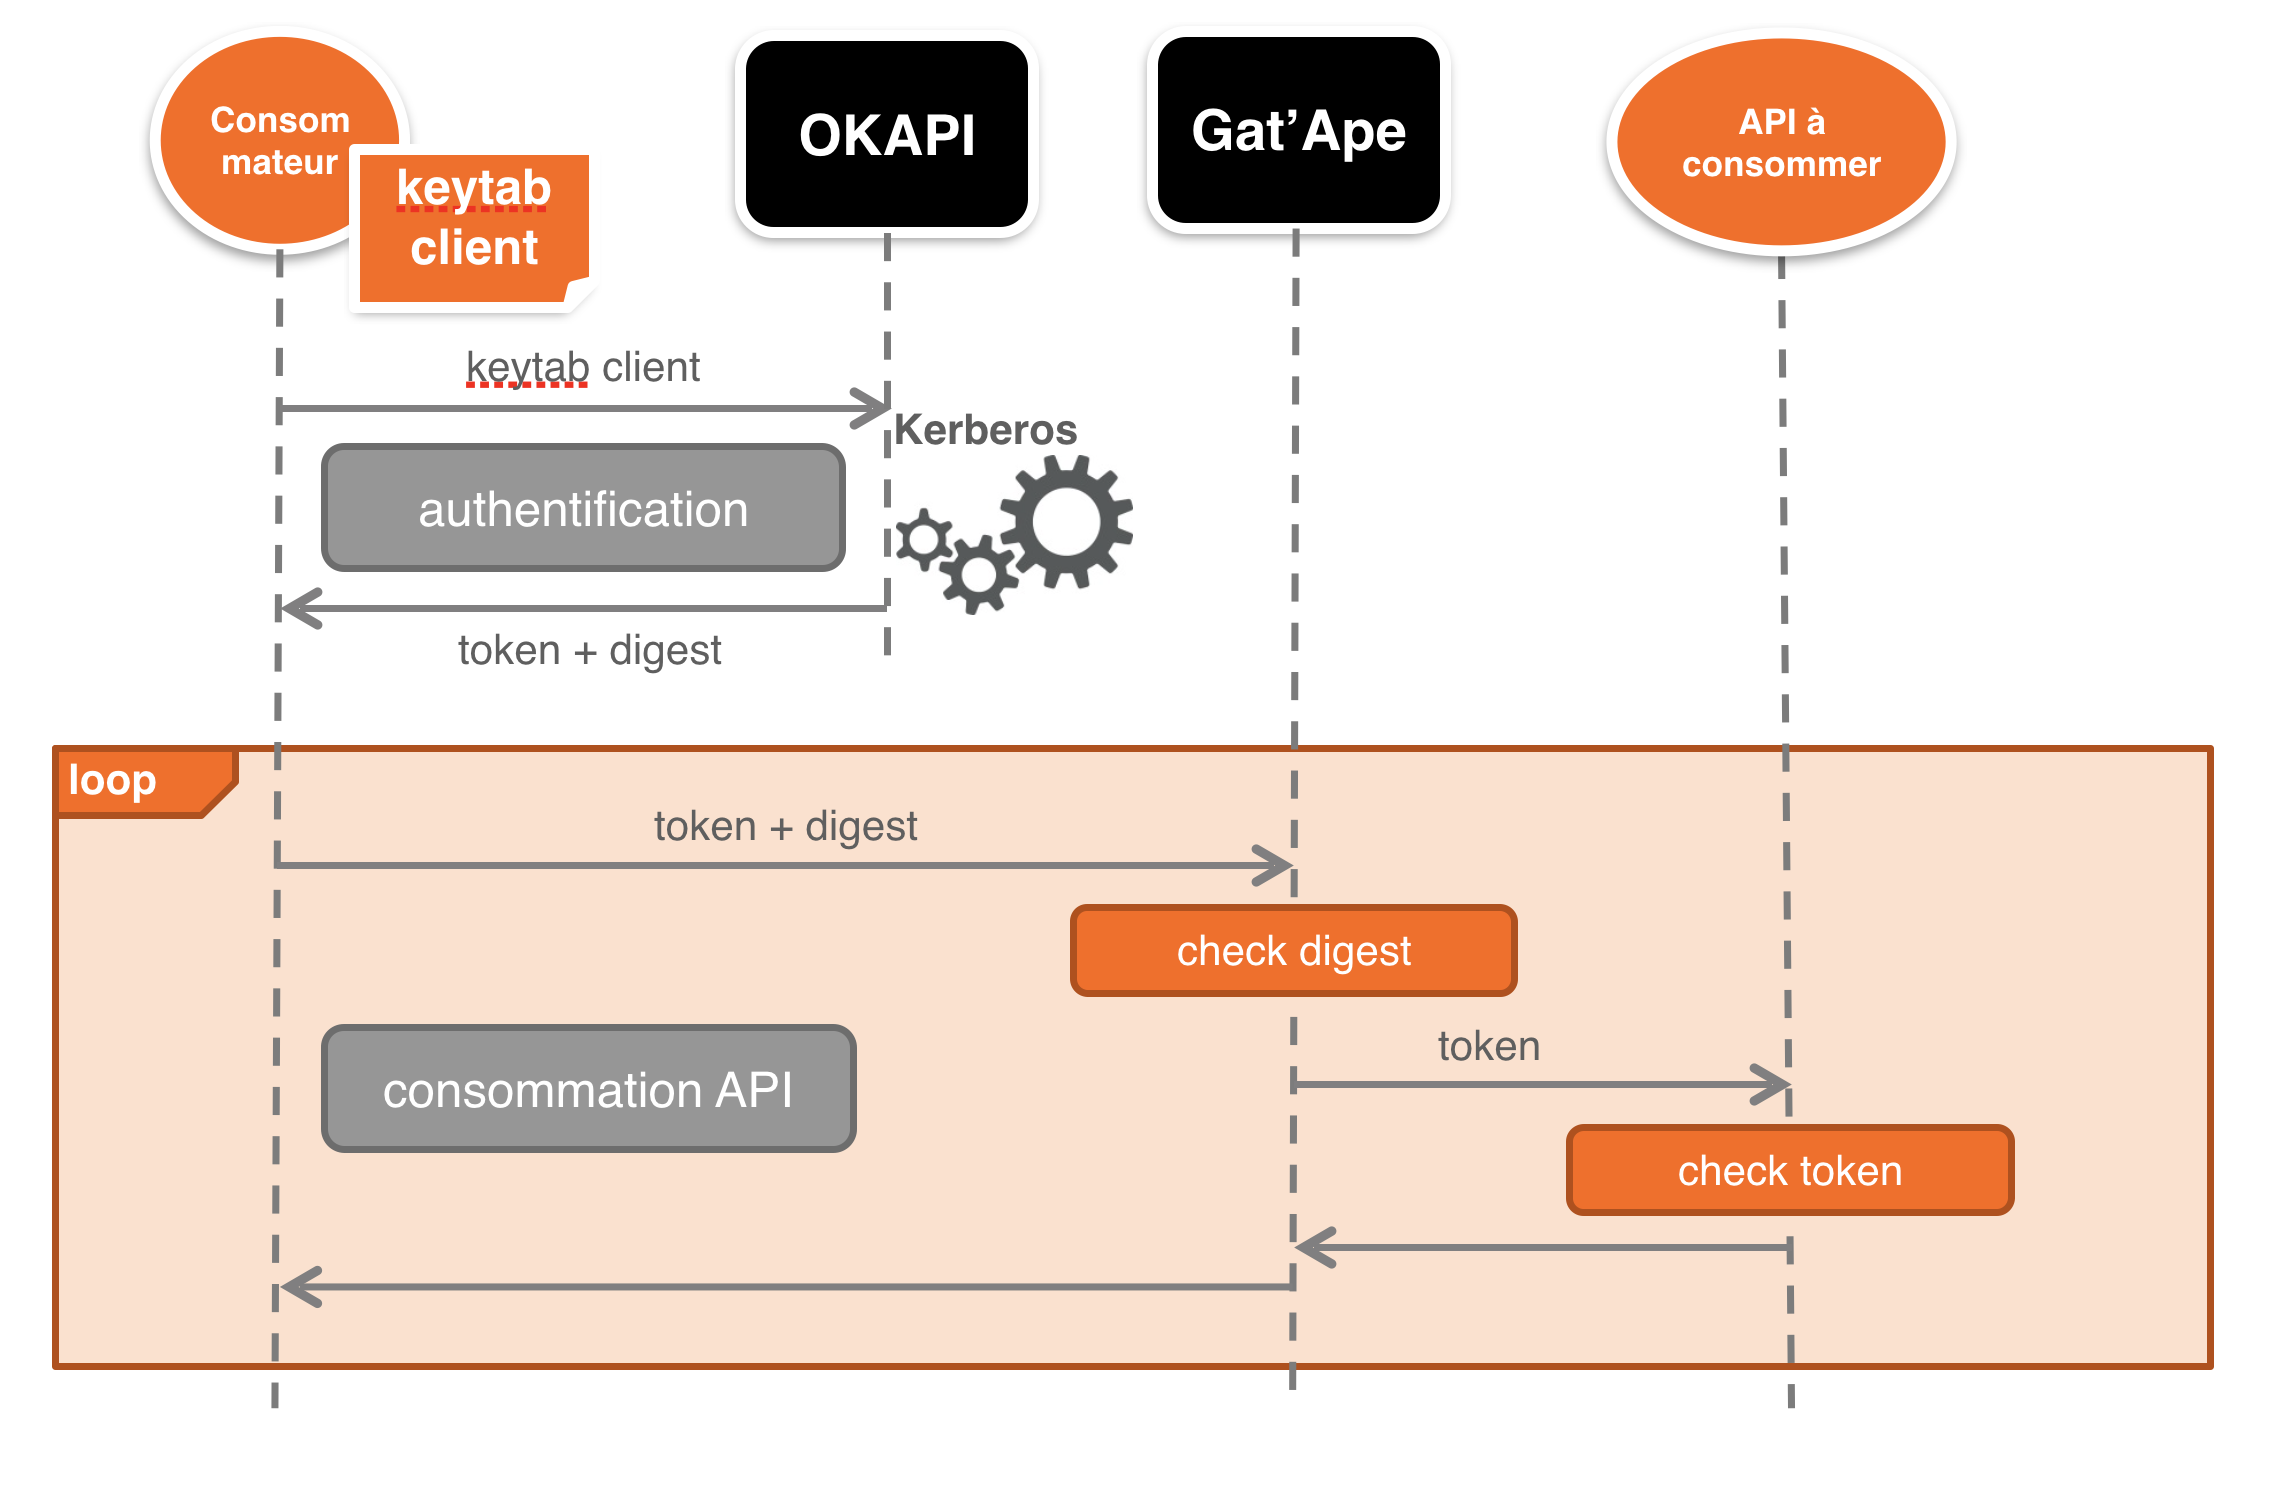
\includegraphics[width=15cm]{images/gao/gao1}
  \caption{Fonctionnement de Gat'Ape/Okapi.}
  \label{gatape}
\end{figure}


Dans les faits la connexion grâce à Gat'ape/okapi se passe comme suit : 
L'application qui vient se connecter possède une clé secrète. Cette clé secrète est envoyée à Okapi. Lors du traitement, Okapi va renvoyer un jeton d'authentification unique au consommateur ainsi qu'un digest. Ceci est la phase d'authentification.  Ce digest est ensuite envoyé du consommateur vers Gat'ape. Si le digest est valide, le consommateur va envoyer le jeton précédemment obtenu vers l'API à laquelle il souhaitait se connecter. L'API va à son tour vérifier le jeton puis le renvoyer ainsi que les informations demandées par le consommateur. Ces informations lui seront transmises via Gat'ape. Si une de ces vérifications de jeton échoue, le protocole recommence un envoi de jeton. L'opération peut ainsi être réitérée un certain nombre de fois sans avoir à se ré authentifier. Cette durée de vie (TTL) est paramétrable.




\subsection{Production}
Avant de commencer la production à proprement parlé j'ai tout d'abord du lire la documentation relative à cette API pour en comprendre l'utilité et le fonctionnement. Une fois que la fonction et le fonctionnement de cette API m'était plus clair, j'ai pris rendez vous avec le responsable solution de cette API. Nous avons fait une réunion dans laquelle je lui ai demandé les points qu'il voulait mettre en avant grâce à la vidéo et les principales innovations qu'apportait Gat'ape/okapi par rapport à l'ancienne solution. Une fois d'accord sur les points à aborder je me suis mis à produire un script, et un storyboard qui sont respectivement le texte de la vidéo et les images et animations clefs de celle ci. Une fois le script et le storyboard finalisé, j'ai de nouveau rencontré le responsable de Gat'ape/Okapi pour les lui proposer. Une fois ces documents validés, j'ai pu me lancer dans la production à proprement parler. \\

Au lancement de la vidéo, les logos de Gat'ape et Okapi arrivent depuis chaque côté de l'écran, présentant ainsi les deux APIs. La partie suivante de la vidéo explique brièvement la fonction générale de Gat'ape/Okapi. Pour cette première partie j'ai voulu expliquer simplement et en quelques secondes à quoi servait Gat'ape/Okapi.  Les APIs exposés au travers de Gat'ape apparaissent en premier, pour symboliser le fait qu'elles sont déjà présentes et visibles, puis les consommateurs font leur apparition et ces derniers sont reliés aux APIs via des flèches en passant par le duo Gat'ape/Okapi.\\

Vient ensuite l'explication de l'identification. Le nom du protocole d'authentification, Okapi, apparaît et est décomposé pour expliquer son acronyme. Dans un premier temps le protocole Oauth2 est expliqué comme étant le moyen de mise en relation du consommateur avec Okapi,  puis Kerberos est succinctement expliqué comme étant un protocole d'identification à base de clé secrète et de jeton. Kerberos étant crucial et complexe, j'ai choisi de l'expliciter dans la partie suivante de la vidéo autour d'une situation connue de tous, l'accès à une salle de cinéma.\\

Dans un premier temps le spectateur, dans le cas concret : le consommateur, va récupérer au guichet (Okapi) son ticket. Une fois ceci fait, le spectateur doit passer devant l'ouvreur au point d'accès de la salle qui va déchirer le ticket et en garder une partie. Lors du contrôle (l'accès à Gat'ape), il est vérifié que les deux morceaux de tickets vont bien ensemble, si c'est le cas le spectateur peut accéder à sa séance (Le consommateur peut accéder à l'API). Il est ensuite précisé que le ticket à une durée bien définie, une séance dans le cas d'un ticket de cinéma, un Time To Live (durée de vie) paramétrable dans le cas de Gat'ape/Okapi.\\

\begin{figure}[htp]
  \centering
  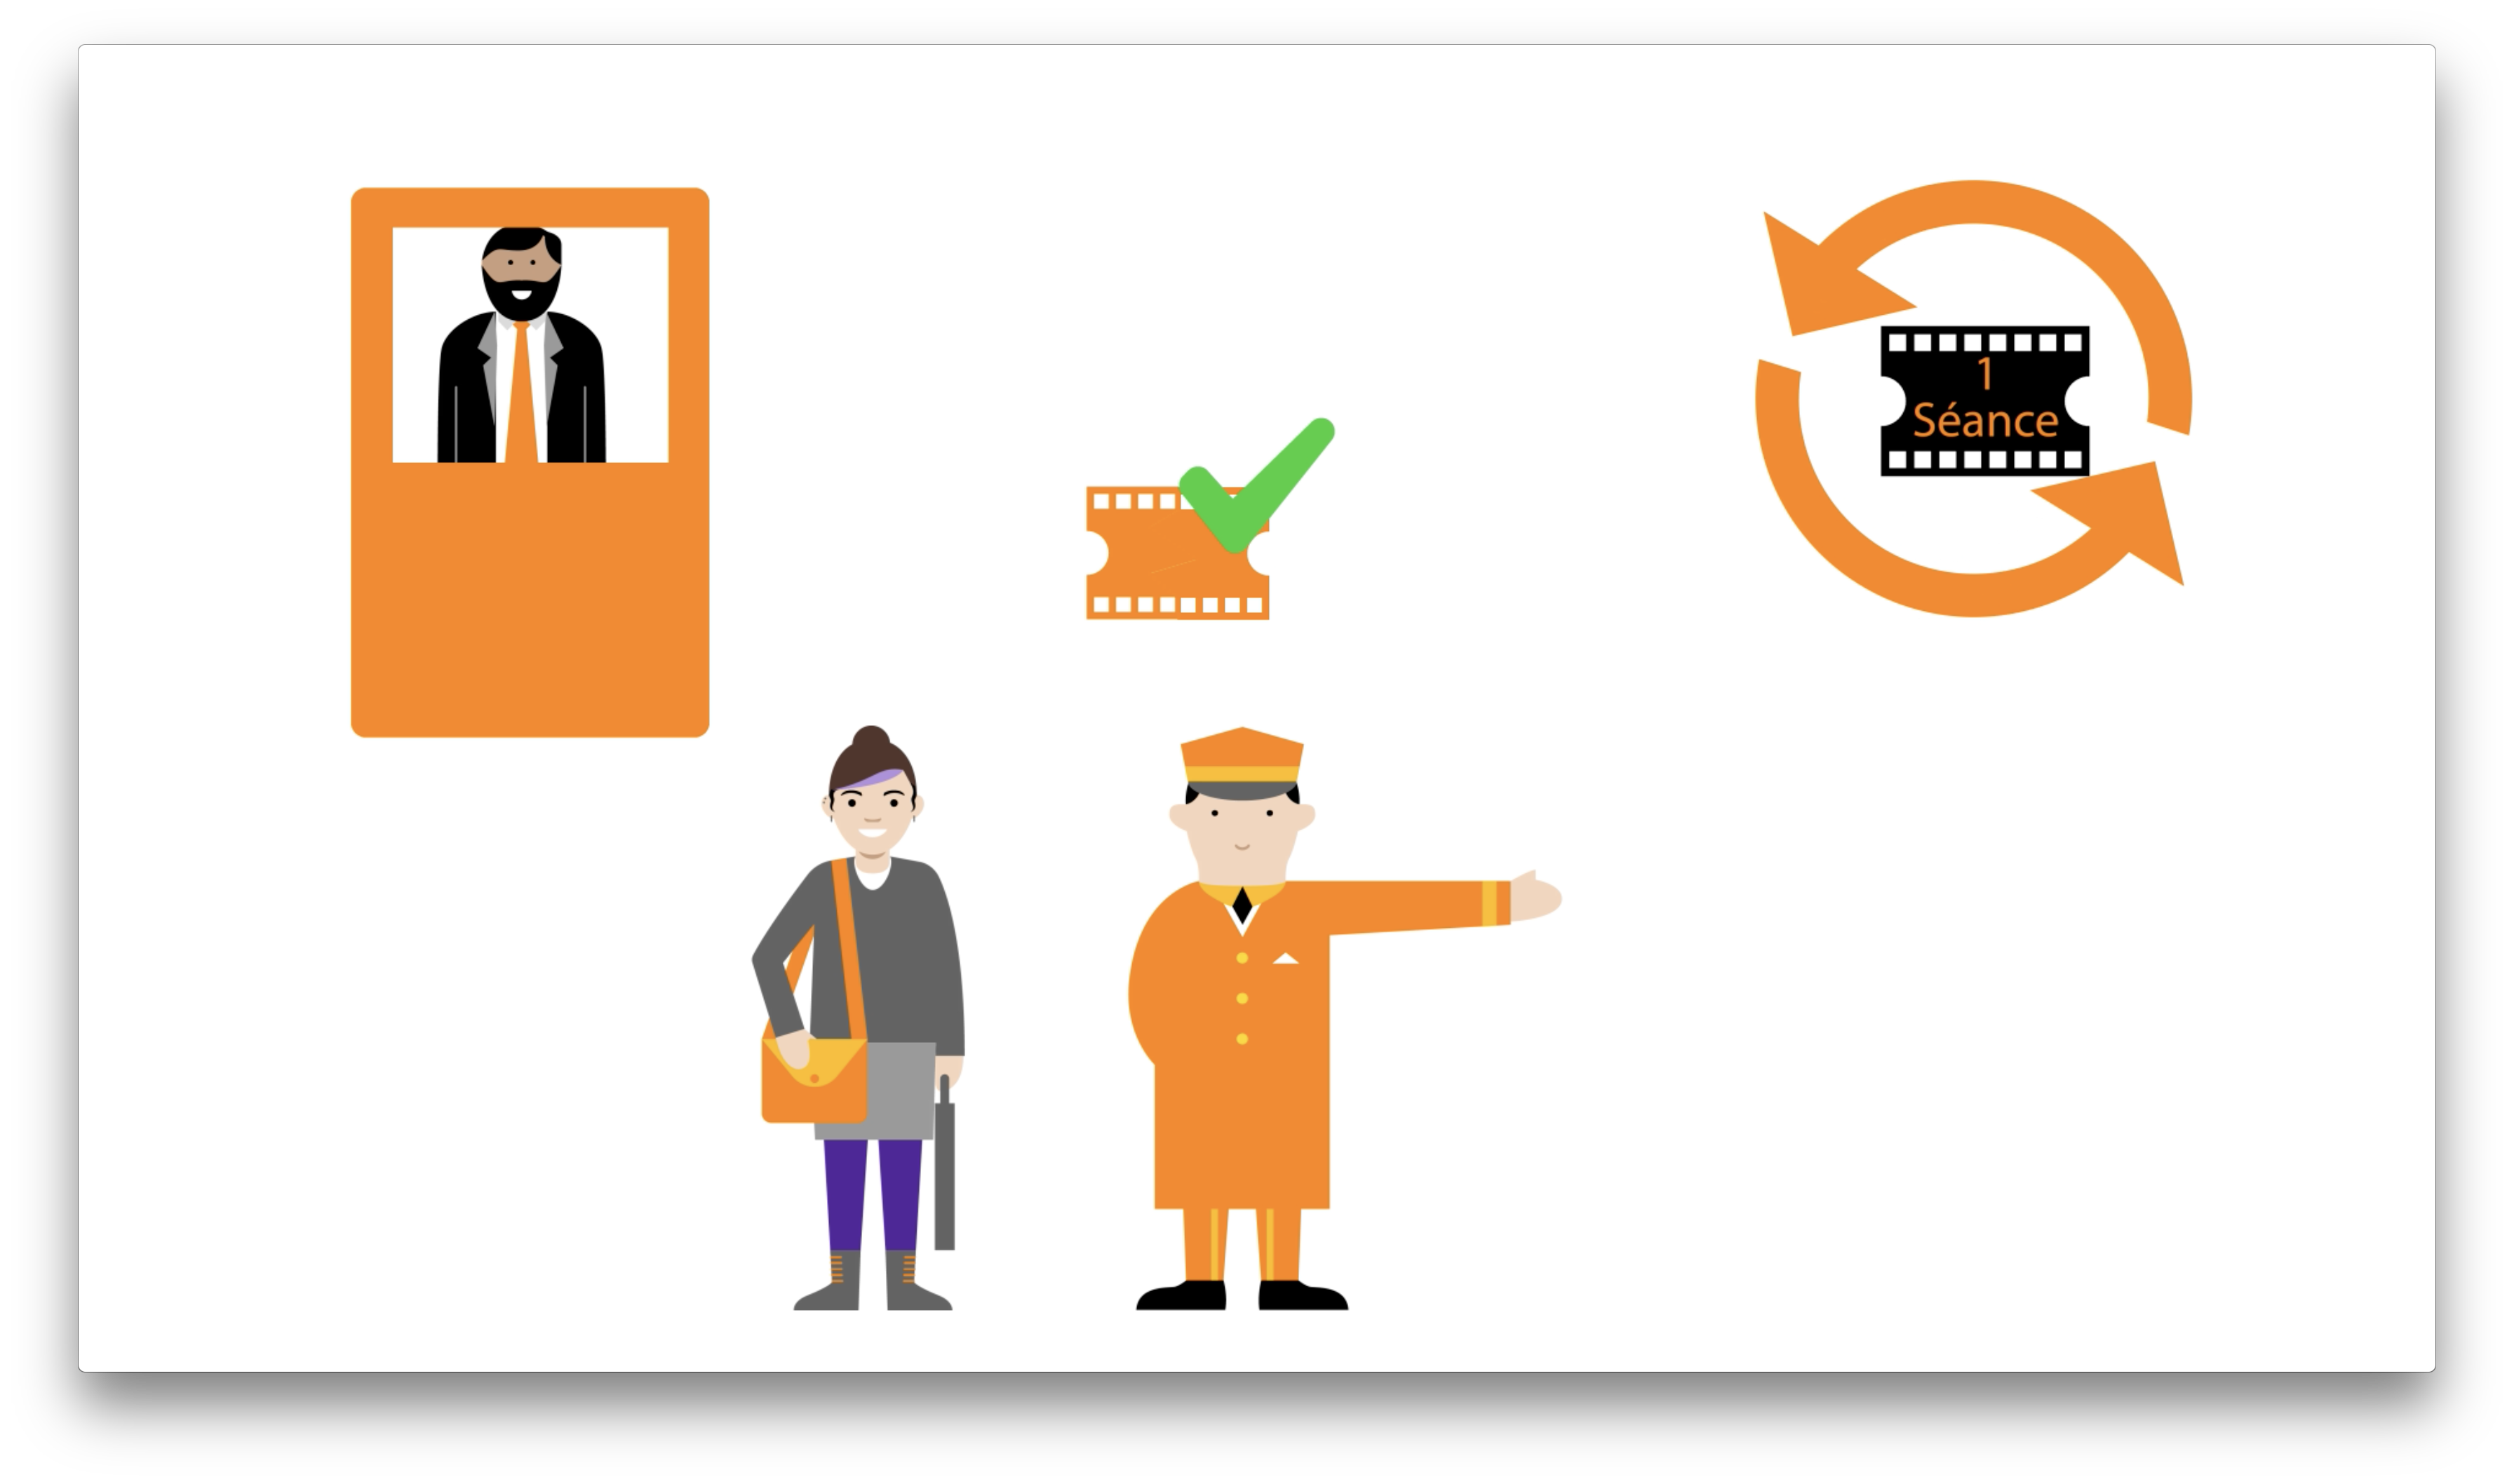
\includegraphics[width=15cm]{images/gao/screenGao}
  \caption{Explication de Kerberos.}
  \label{screengatape}
\end{figure}

Il est ensuite mis en avant les possibilités qu'offre Gat'ape dans la mise en relation entre le consommateur et l'API, tels le contrôle d'accès, qui va permettre d'autoriser ou non l'accès à une API à certains consommateurs et le contrôle de trafic qui va permettre de réguler les flux d'accès en fonction de la demande des consommateurs et de la disponibilité de l'api. Pour représenter le contrôle d'accès j'ai choisi d'utiliser des croix rouges et des coches vertes afin de rester simple et compréhensible. J'ai choisi d'illustrer le contrôle de trafic avec des feux tricolores que l'on voit changer de couleur pour symboliser le fait que ce contrôle n'est pas figé et se déroule en continu. La fonctionnalité mise en avant ensuite est la détection d'erreurs et d'anomalies qui est fournie par une autre API intégrée à Gat'ape, représentée par un moniteur qui contient une sorte d'électrocardiogramme qui grandit dangereusement à un moment, cette anomalie est ensuite entourée en rouge avec un panneau danger, qui représente la détection.\\

Les fonctionnalité mentionnées ensuite sont un surcoût de temps de réponse quasi nul, qui n'impacte pas les performances, et une architecture tri site, qui assure  une très haute disponibilité. En effet, si l'un des trois sites venait à subir une maintenance, une attaque ou être indisponible pour une autre raison, il y a deux autres sites qui pourront fournir l'authentification et garantir la sécurité aux consommateurs.\\

La dernière section de la vidéo n'était pas prévue dans le storyboard d'origine mais la vidéo étant un peu longue et assez détaillée sur certains points, et les personnes les moins techniques pourraient avoir décroché. J'ai donc choisi ici de faire un rapide résumé de la situation en rajoutant l'information qu'il existe un SDK pour permettre l'intégration facile de Gat'ape/Okapi à son application et qu'il existe un modèle d'API contenant Gat'ape/okapi prêt à l'usage pour les personnes souhaitant développer une API. Dans la dernière séquence, sont indiqués les liens vers la documentation et le mail de l'équipe en charge pour les personnes souhaitant avoir plus d'informations à ce sujet. 



\section{Vidéo sur Zbus}

\subsection{Contexte}
Zbus est une API permettant le transfert de messages au fil de l'eau entre les applications du SI. Zbus à pour but de faciliter et standardiser l'alimentation de Push@voo, qui est la plate forme permettant d'envoyer les notifications,  comme par exemple le nombre de mails non lus. L'API Zbus fonctionne sur un modèle de publish/subscribe : les messages sont classés par catégorie auxquelles s'abonnent les récepteurs. Les messages sont donc en attente active ou "polling" et ne sont délivrés qu'une seule fois. Chaque récepteur à sa propre file d'attente qui sera donc remplie avec les messages dont les catégories l'intéresse dans l'ordre d'arrivée.  


\subsection{Production}

Une fois d'accord sur le storyboard avec le responsable de l'API, j'ai commené la réalisation. Comme pour la vidéo précédente, l'ouverture se fait avec le logo de l'Zbus qui arrive à l'écran puis disparaît. Lors de la séquence suivante, la fonction de l'API est résumée très brièvement en tant que la composante qui permet l'envoi de notification, ce qui est, entre autre, une de ses fonctions. J'ai choisi cette facette de Zbus car elle est très facilement compréhensible et visualisable. L'animation par dessus la voix off est donc une enveloppe qui arrive et une notification ronde qui apparaît pour signifier qu'un nouveau message est arrivé.\\

Vient ensuite les explications sur le fonctionnement de l'API. Pour symboliser le fait que les récepteurs s'abonnent au fil de messages, ils sont reliés par un trait à l'émetteur en forme de nuage. On voit ensuite à quelles catégories de messages chaque récepteur c'est abonné sur son écran. Ici pour des raisons de simplicité, les catégories de messages sont représentés par trois couleurs : bleu, rouge et vert. Un des récepteurs est abonné aux trois catégories de messages, un autre à seulement deux catégories et le troisième n'est abonné qu'à la catégorie bleue. Ensuite, la file d'attente de chaque récepteur apparaît à côté de lui et l'émetteur commence à envoyer des messages. 


\begin{figure}[htp]
  \centering
  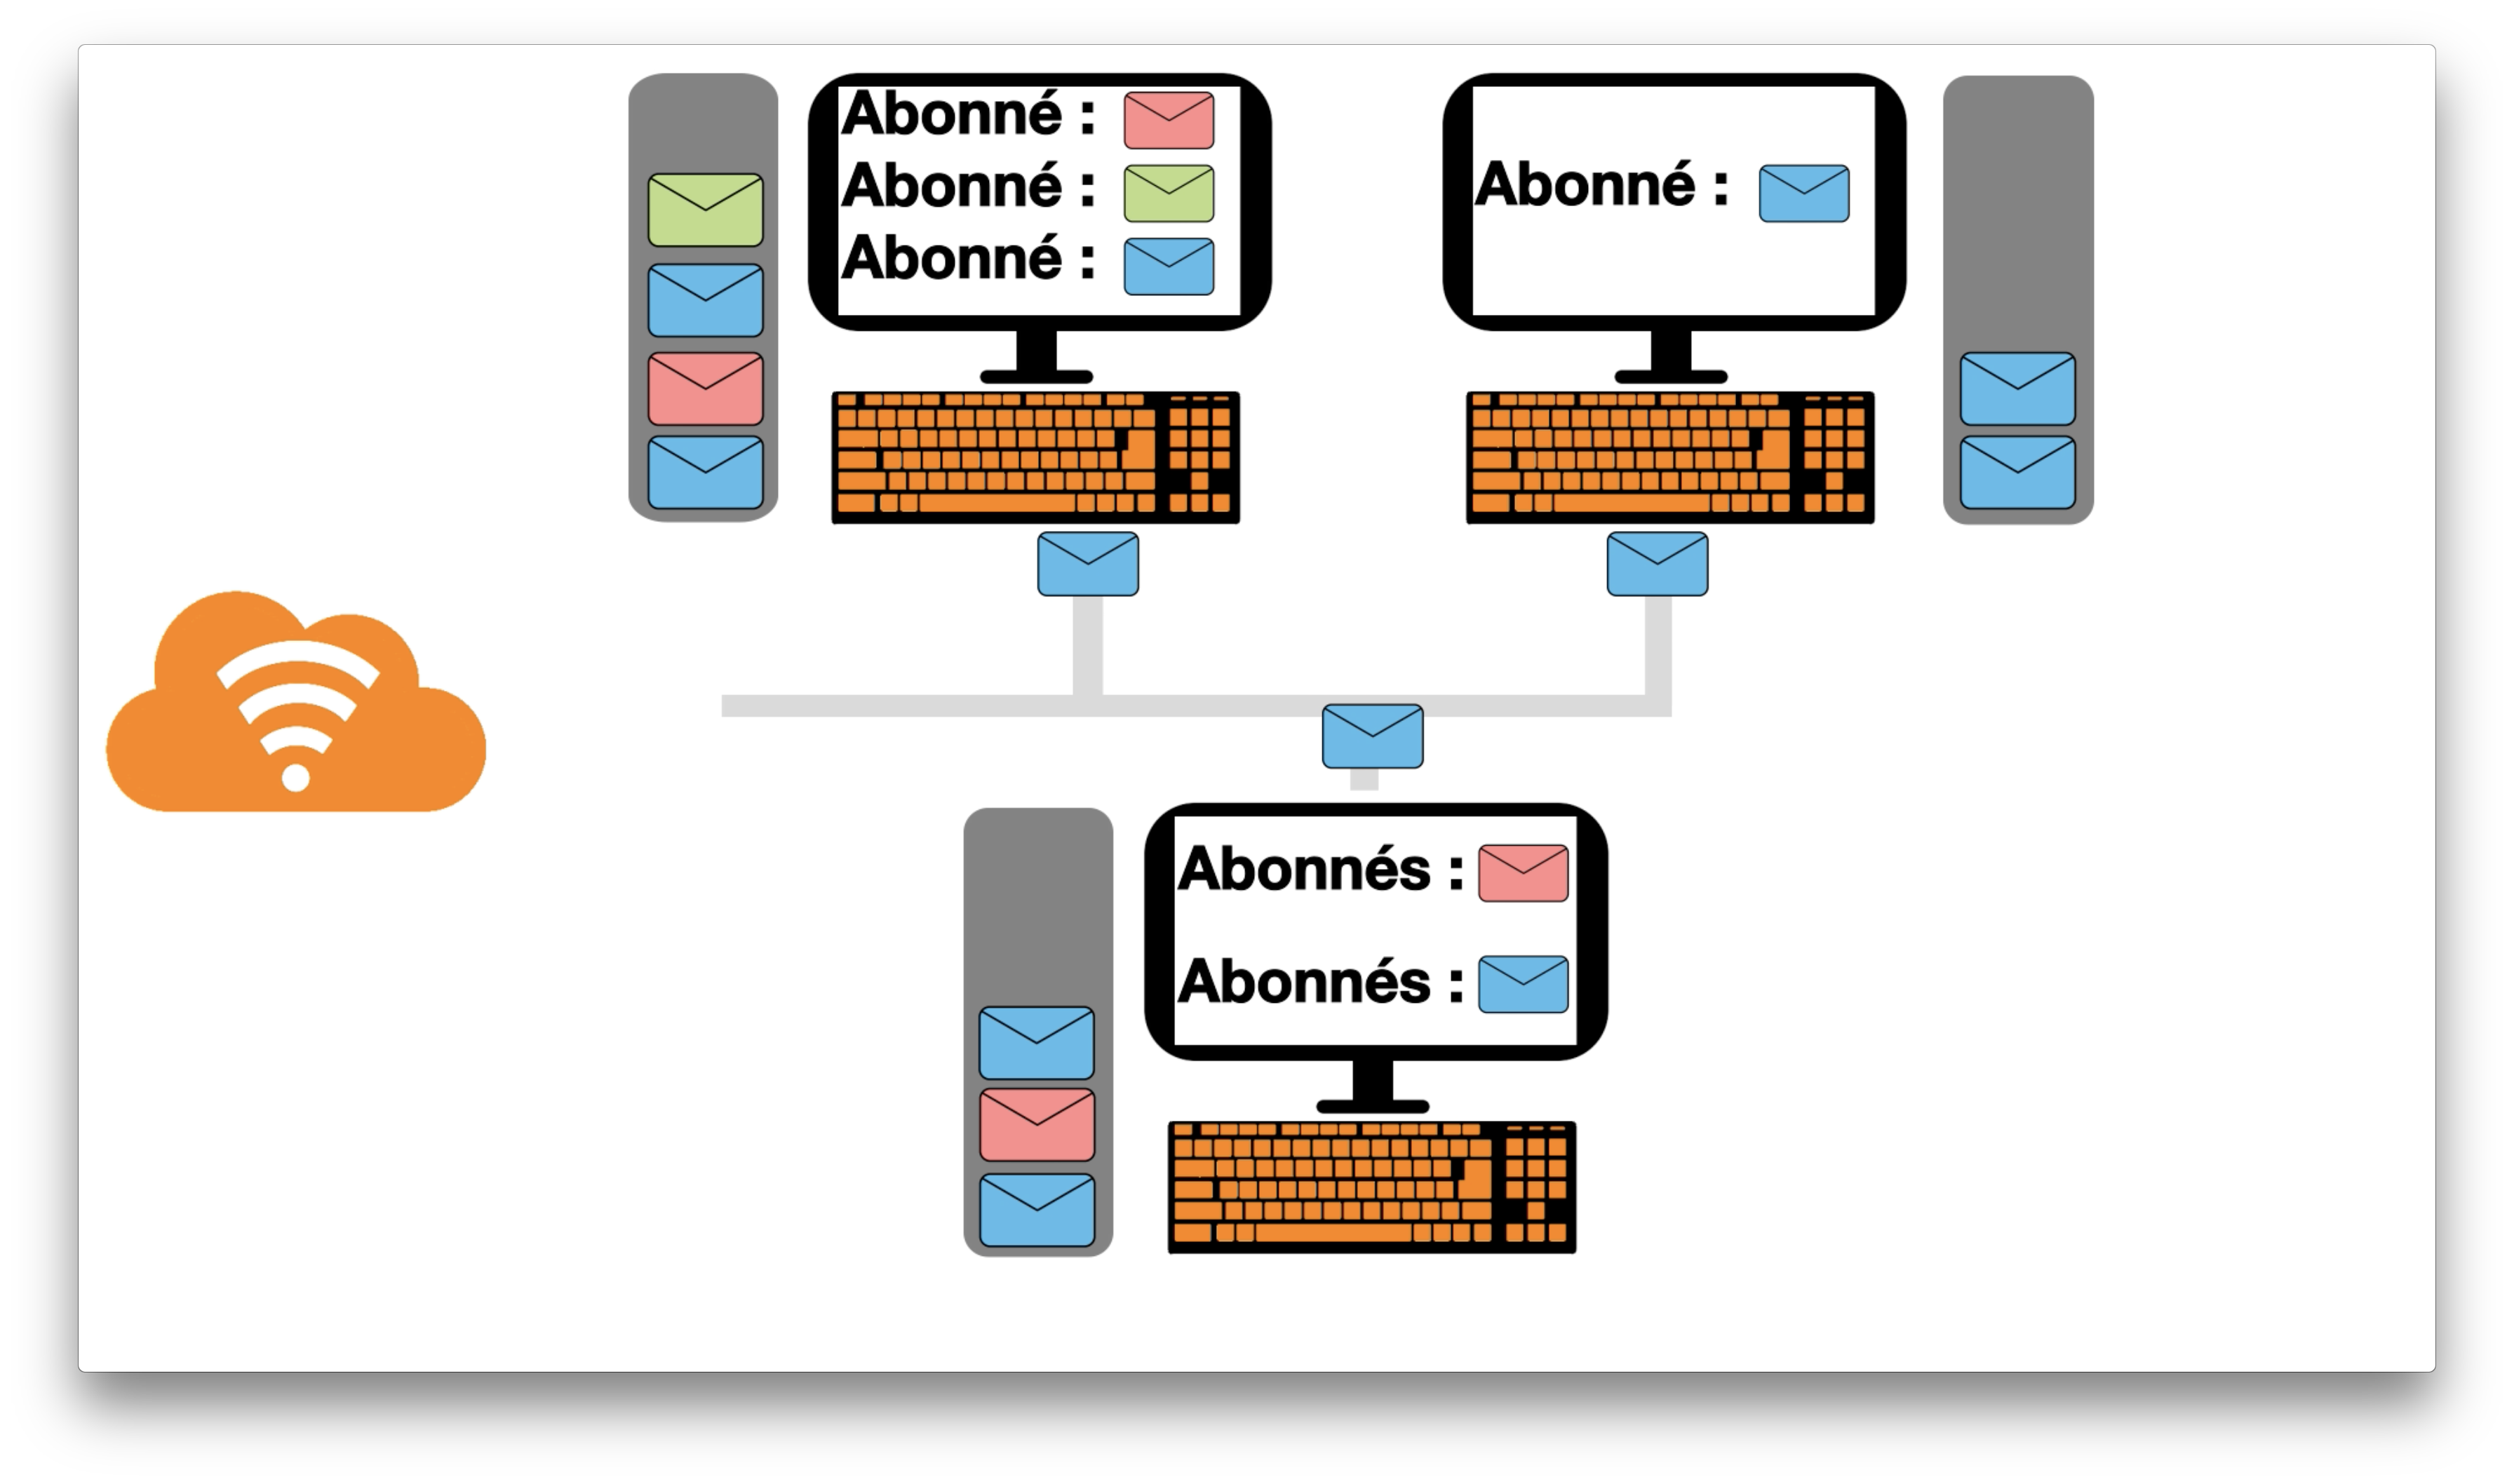
\includegraphics[width=15cm]{images/zbus/screensbus.png}
  \caption{Les files d'attentes dans Zbus.}
  \label{screenzbus}
\end{figure}


Un message est émis une seule fois puis sera intercepté par les récepteurs abonnés à cette catégorie puis stocké dans leur file d'attente en attendant d'être traité. A la fin de cette séquence, chaque récepteur a bien dans sa file des messages correspondant à ce dont ils s'étaient abonnés.\\

La séquence suivante évoque les types de fihiers qui peuvent être échangés via Zbbus. L'animation correspond tout simplement au changement de mot au moment de la parole.\\

Puis vient une animation expliquant les avantages de Zbus qui sont sa facilité d'utilisation et sa sécurité. Les logos décendent depuis un trait situé entre une fenêtre d'application et le logo de Zbbus. Ce logo va ensuite se décaler et cohaiter à l'écran avec le logo de Push@voo. Une enveloppe va circuler de Zbus vers Push@voo puis des notifications rondes vont ensuite apparaître, expliquant une nouvelle fois que Zbus fonctionne de pair avec Push@voo pour permettre l'envoi de notifications.\\

Enfin, nous retrouvons une séquence classique qui contient les liens intranets vers la documentation et le mail de l'équipe de Zbus.


\section{Vidép sur Valkey}

\subsection{Contexte}

\subsection{Production}




\section{Le cloud chez Orange (Comité de direction)}
\subsection{Contexte}
Le 12 juin 2016, Koen Vermeulen, CIO d'Orange ainsi que son comité de direction sont venus sur le site de Sophia-Antioplis dans le but de voir les avancements du cloud et de comment celui ci pouvait impacter la totalité d'Orange et pas seulement les développeurs axés sur les nouvelles technologies comme c'est la cas à la DFY. Un créneau de démonstration à donc été réservé pour une équipe qui devait montrer les différentes étapes avant et après l'arrivée du cloud pour un développeur qui souhaite créer une application se connectant à la base de donnée.\\

J'ai donc été missionné pour la première partie de cette intervention en ayant pour but de "produire une vidéo de moins de 3 minutes expliquant le côté laborieux pour un développeur de déployer une application depuis avec les étapes de demande de machines, flux, connexion au backend".\\

Cette vidéo fut suivi d'une démonstration d'un déploiement d'une API en obtenant automatiquement les identifiants de connection.

\subsection{Réalisation}
Avant de réaliser le storyboard, j'ai du rencontrer les deux développeurs qui s'occupaient de la démonstration qui se passait juste après ma vidéo dans le but de savoir sur quels point je devais appuyer afin que leur démonstration fasse bien contraste avec la situation précédente. Les points qui sont ressortis sont

\begin{itemize}
    \item Le temps à attendre avant la mise en service
    \item Les formulaires à remplir manuellement qui transitaient de main en main
    \item La nécessité de passer par des services externes
\end{itemize}


\begin{figure}[htp]
  \centering
  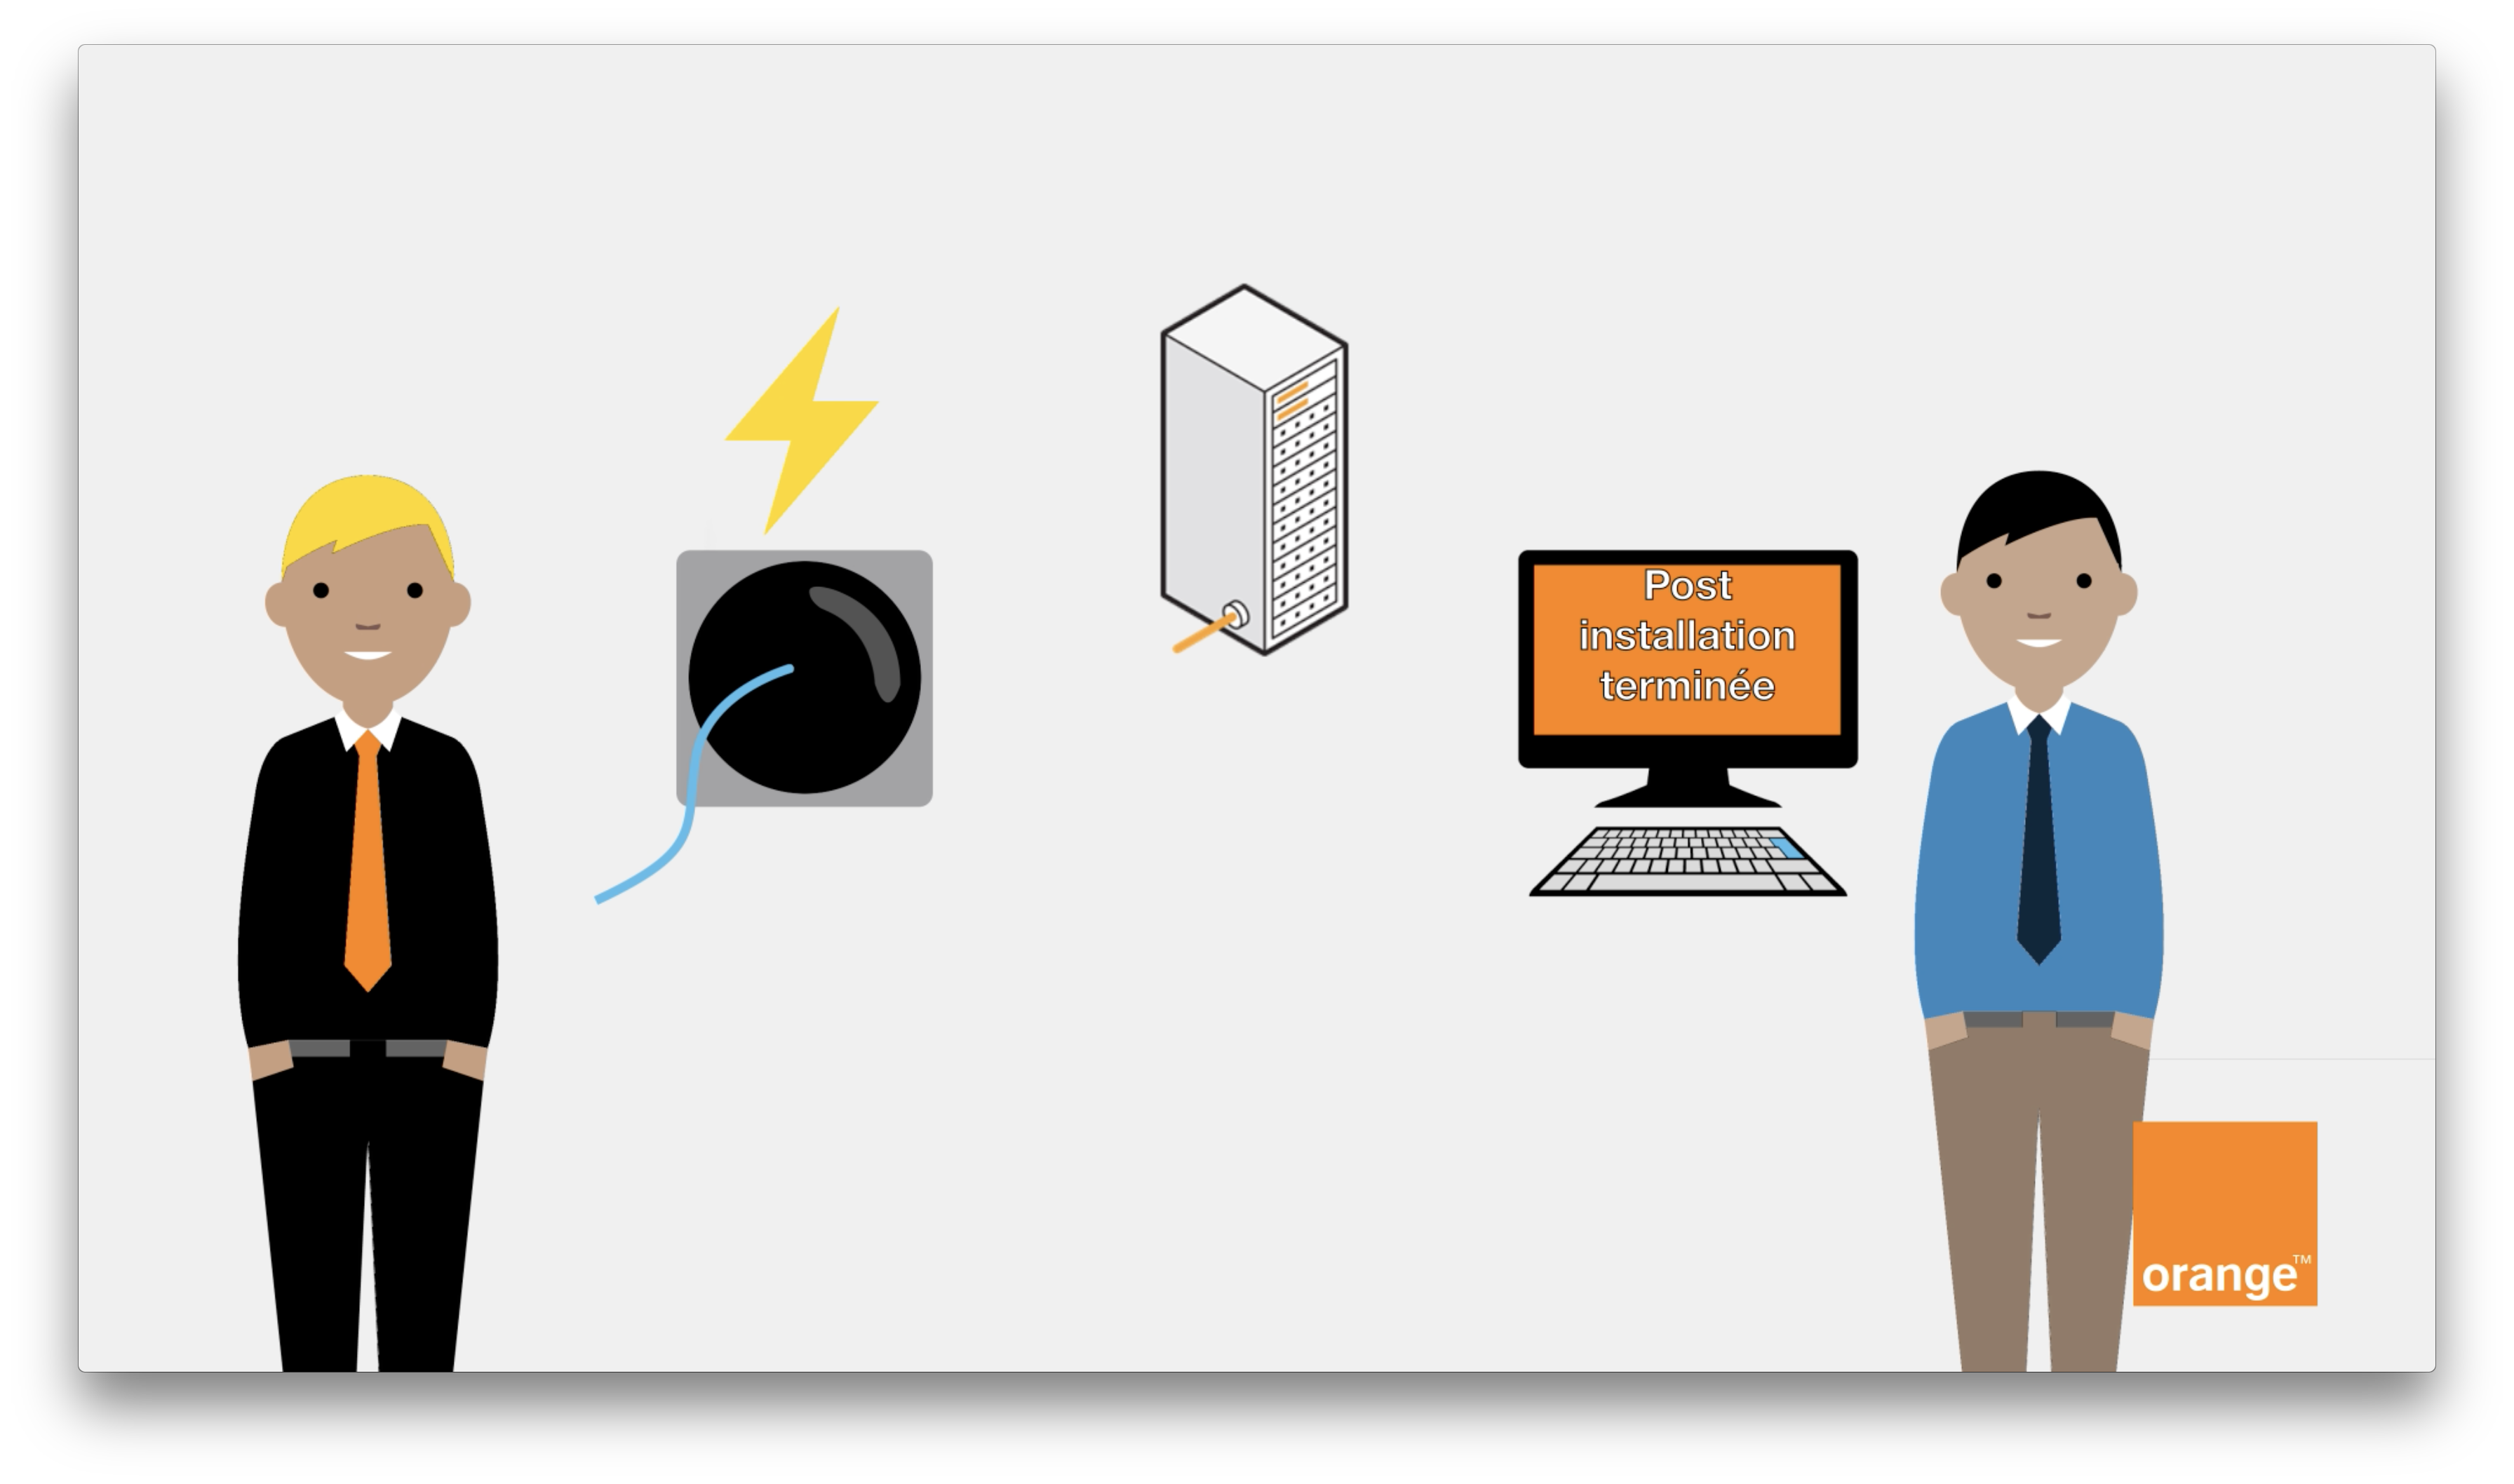
\includegraphics[width=15cm]{images/cd/cd.png}
  \caption{Les étapes de l'installationavant la mise en place du cloud.}
  \label{comite}
\end{figure}



\section{Présentation de PnS.com (Comité d'investissement)}
\subsection{Contexte}

\subsection{Réalisation}


\section{Présentation du devops}
\subsection{Contexte}

\subsection{Réalisation}


\section{Newsletter}

%%% Local Variables: 
%%% mode: latex
%%% TeX-master: "isae-report-template"
%%% End: 

%%% .warn @Kyuu ��#2146  fais gaffe à ton langage quand même
\chapter*{Conclusion et perspectives}
\addcontentsline{toc}{chapter}{Conclusion}
\markboth{Conclusion}{Conclusion}
\label{sec:conclusion}

Au long de ces six mois de stage passés sur le site d'Orange de Sophia-Antipolis, j'ai pu découvrir un métier aux enjeux variés allant de l'explication de technologies en interne à 
l'explication de méthodes de travail qui ciblera des personnes en dehors de l'entreprise. 
J'ai particulièrement apprécié la liberté de création qui m'a été accordée pour la réalisation des vidéos, même si j'aurais aimé bénéficier de plus de temps pour pouvoir créer moi même la totalité des illustrations. J'ai aussi dû approfondir mes connaissances du logiciel After Effect utilisé pour le montage pour pouvoir produire des effets de transitions que nous n'avions pas eu le temps de réaliser dans les cours de pratiques plastiques. Ce stage m'aura permis de confirmer que les missions créatives sont les plus adaptées pour moi, mais qu'il ne faut pas non plus négliger l'aspect technique qui reste très présent.\\

La DFY m’a accueilli pendant une période charnière : son passage aux APIs via le cloud, et je suis fier d’avoir pu prendre part à ce changement qui va permettre une facilité d'intégration des applications et l'accès aux données ainsi qu'à la sécurisation des échanges qui est un paramètre plus qu'important de nos jours. J'ai notamment étoffé mes connaissances sur la sécurité et les étapes de créations d'une application qui change ne nos habitudes universitaires. En effet là où nous commençons chaque application à partir de rien, celles de la DFY sont construites à partir de briques pré-établies. Les connaissances acquises au cours de mon cursus m'ont permis de comprendre le fonctionnement de la plupart des composantes de l'écosystème PnS.\\

Suite à cette expérience, je souhaite m'orienter dans un secteur qui soit aussi technologique et innovant que celui dans lequel j'ai effectué ce stage et dans lequel il y aurait toujours une part importante de créativité.


%%% Local Variables: 
%%% mode: latex
%%% TeX-master: "isae-report-template"
%%% End: 



\appendix

\bibliographystyle{authoryear-fr}
\bibliography{references}

\clearpage

%%%%%%%%%%%%%%%%
%%% Abstract %%%
%%%%%%%%%%%%%%%%

\thispagestyle{empty}

\vspace*{\fill}
\noindent\rule[2pt]{\textwidth}{0.5pt}\\


\noindent\rule[2pt]{\textwidth}{0.5pt}
\begin{center}
  Orange\\
  790 Avenue Maurice Donat\\
  06250 Mougins
\end{center}
\vspace*{\fill}

\end{document}